% Options for packages loaded elsewhere
\PassOptionsToPackage{unicode}{hyperref}
\PassOptionsToPackage{hyphens}{url}
\PassOptionsToPackage{dvipsnames,svgnames,x11names}{xcolor}
%
\documentclass[
  11pt,
]{article}
\usepackage{amsmath,amssymb}
\usepackage{iftex}
\ifPDFTeX
  \usepackage[T1]{fontenc}
  \usepackage[utf8]{inputenc}
  \usepackage{textcomp} % provide euro and other symbols
\else % if luatex or xetex
  \usepackage{unicode-math} % this also loads fontspec
  \defaultfontfeatures{Scale=MatchLowercase}
  \defaultfontfeatures[\rmfamily]{Ligatures=TeX,Scale=1}
\fi
\usepackage{lmodern}
\ifPDFTeX\else
  % xetex/luatex font selection
\fi
% Use upquote if available, for straight quotes in verbatim environments
\IfFileExists{upquote.sty}{\usepackage{upquote}}{}
\IfFileExists{microtype.sty}{% use microtype if available
  \usepackage[]{microtype}
  \UseMicrotypeSet[protrusion]{basicmath} % disable protrusion for tt fonts
}{}
\makeatletter
\@ifundefined{KOMAClassName}{% if non-KOMA class
  \IfFileExists{parskip.sty}{%
    \usepackage{parskip}
  }{% else
    \setlength{\parindent}{0pt}
    \setlength{\parskip}{6pt plus 2pt minus 1pt}}
}{% if KOMA class
  \KOMAoptions{parskip=half}}
\makeatother
\usepackage{xcolor}
\usepackage[letterpaper,margin=0.78in]{geometry}
\usepackage{longtable,booktabs,array}
\usepackage{calc} % for calculating minipage widths
% Correct order of tables after \paragraph or \subparagraph
\usepackage{etoolbox}
\makeatletter
\patchcmd\longtable{\par}{\if@noskipsec\mbox{}\fi\par}{}{}
\makeatother
% Allow footnotes in longtable head/foot
\IfFileExists{footnotehyper.sty}{\usepackage{footnotehyper}}{\usepackage{footnote}}
\makesavenoteenv{longtable}
\usepackage{graphicx}
\makeatletter
\def\maxwidth{\ifdim\Gin@nat@width>\linewidth\linewidth\else\Gin@nat@width\fi}
\def\maxheight{\ifdim\Gin@nat@height>\textheight\textheight\else\Gin@nat@height\fi}
\makeatother
% Scale images if necessary, so that they will not overflow the page
% margins by default, and it is still possible to overwrite the defaults
% using explicit options in \includegraphics[width, height, ...]{}
\setkeys{Gin}{width=\maxwidth,height=\maxheight,keepaspectratio}
% Set default figure placement to htbp
\makeatletter
\def\fps@figure{htbp}
\makeatother
\setlength{\emergencystretch}{3em} % prevent overfull lines
\providecommand{\tightlist}{%
  \setlength{\itemsep}{0pt}\setlength{\parskip}{0pt}}
\setcounter{secnumdepth}{-\maxdimen} % remove section numbering
\usepackage{fontspec,microtype,booktabs,longtable,array,tabularx}
\usepackage{tikz,tcolorbox,fancyhdr,titlesec,caption,xurl,needspace,hyperref}
\usetikzlibrary{calc}
\definecolor{DeepPurple}{HTML}{301356}
\definecolor{RoyalPurple}{HTML}{8051C9}
\definecolor{Lilac}{HTML}{C4A8F0}
\definecolor{PalePurple}{HTML}{F4EFFA}
\definecolor{Ink}{HTML}{201A2A}
\definecolor{Muted}{HTML}{665D70}
\definecolor{AccentGreen}{HTML}{247C68}
\setmainfont{DejaVu Serif}[ItalicFont={Nimbus Roman Italic},BoldItalicFont={Nimbus Roman Bold Italic}]
\setsansfont{DejaVu Sans}
\setmonofont{DejaVu Sans Mono}[Scale=0.78]
\color{Ink}
\setlength{\parindent}{0pt}
\setlength{\parskip}{5.8pt plus 1pt minus 1pt}
\setlength{\emergencystretch}{2.6em}
\setlength{\tabcolsep}{5pt}
\renewcommand{\arraystretch}{1.2}
\titleformat{\section}{\Large\sffamily\bfseries\color{DeepPurple}}{\thesection}{0.65em}{}
\titleformat{\subsection}{\large\sffamily\bfseries\color{DeepPurple}}{\thesubsection}{0.65em}{}
\titleformat{\subsubsection}{\normalsize\sffamily\bfseries\color{DeepPurple}}{\thesubsubsection}{0.65em}{}
\titlespacing*{\section}{0pt}{17pt}{7pt}
\titlespacing*{\subsection}{0pt}{13pt}{5pt}
\captionsetup{font=small,labelfont={bf,color=DeepPurple},justification=raggedright,singlelinecheck=false}
\hypersetup{colorlinks=true,linkcolor=DeepPurple,urlcolor=RoyalPurple,citecolor=DeepPurple,
pdftitle={🌌♾️ AGI ALPHA FLYWHEEL — When Capability Creates Opportunity},
pdfauthor={Vincent Boucher — President of MONTREAL.AI},
pdfsubject={A bounded discovery campaign, exact finite constructions, prior-art comparisons and conditional economics},
pdfkeywords={AGI ALPHA, opportunity discovery, passive chronology, novelty gate, finite-model evidence}}
\pagestyle{fancy}
\fancyhf{}
\fancyhead[L]{\scriptsize\sffamily\color{DeepPurple}AGI ALPHA FLYWHEEL}
\fancyhead[R]{\scriptsize\sffamily\color{Muted}WHEN CAPABILITY CREATES OPPORTUNITY}
\fancyfoot[L]{\scriptsize\sffamily\color{Muted}MONTREAL.AI \quad Research edition 01 \quad 27 October 2026}
\fancyfoot[R]{\small\sffamily\color{DeepPurple}\thepage}
\renewcommand{\headrulewidth}{0.25pt}
\setlength{\headheight}{15pt}
\setlength{\headsep}{20pt}
\setlength{\footskip}{29pt}
\let\oldquote\quote
\let\endoldquote\endquote
\renewenvironment{quote}{\begin{tcolorbox}[colback=PalePurple,colframe=Lilac,boxrule=0.45pt,arc=2pt,left=10pt,right=10pt,top=7pt,bottom=7pt]}{\end{tcolorbox}}
\ifLuaTeX
  \usepackage{selnolig}  % disable illegal ligatures
\fi
\IfFileExists{bookmark.sty}{\usepackage{bookmark}}{\usepackage{hyperref}}
\IfFileExists{xurl.sty}{\usepackage{xurl}}{} % add URL line breaks if available
\urlstyle{same}
\hypersetup{
  colorlinks=true,
  linkcolor={Maroon},
  filecolor={Maroon},
  citecolor={Blue},
  urlcolor={Blue},
  pdfcreator={LaTeX via pandoc}}

\author{}
\date{}

\begin{document}

\begin{titlepage}
\thispagestyle{empty}

\begin{tikzpicture}[remember picture,overlay]
\fill[DeepPurple!76!black] (current page.south west) rectangle (current page.north east);
\begin{scope}[shift={(current page.south west)},x=1in,y=1in]
\foreach \x/\y/\r in {0.4/10.5/.012,1.2/9.7/.008,2.1/10.1/.01,3.7/9.9/.006,4.6/10.4/.01,6.2/10.7/.009,7.8/9.6/.012,7.2/8.2/.008,6.8/7.8/.012,7.7/6.8/.006,5.9/9.1/.006,0.5/8.5/.007,0.35/6.3/.009,7.8/5.4/.01,6.9/5.1/.007,6.3/4.6/.006,7.4/3.7/.01,7.8/2.2/.009,6.5/1.3/.006,5.4/.6/.008,4.2/.4/.01,2.4/.55/.007,1.1/.4/.008,0.4/2.3/.01,0.6/4.3/.006,5.1/8.9/.005,6.1/8.0/.005,7.1/9.1/.005,2.7/10.7/.005,5.2/10.8/.005,7.9/.6/.005}
\fill[white,opacity=.6] (\x,\y) circle[radius=\r];
\draw[Lilac,opacity=.15,line width=1pt] (7.2,9.2) circle[radius=1.55];
\draw[Lilac,opacity=.12,line width=.7pt] (7.2,9.2) ellipse[x radius=1.9,y radius=.55,rotate=25];
\node[text=white,opacity=.16,font=\fontsize{86}{86}\selectfont] at (7.0,9.05) {$\infty$};
\node[anchor=west,text=Lilac,font=\sffamily\small] at (.76,10.28) {MONTREAL.AI \quad / \quad RESEARCH EDITION 01};
\node[anchor=north west,text=white,text width=6.8in,font=\sffamily\bfseries\fontsize{42}{46}\selectfont,align=left] at (.73,8.94) {AGI ALPHA\\FLYWHEEL};
\node[anchor=north west,text=white,text width=6.6in,font=\sffamily\fontsize{24}{29}\selectfont,align=left] at (.77,7.38) {When Capability\\Creates Opportunity};
\node[anchor=north west,text=Lilac,text width=6.45in,font=\sffamily\fontsize{11.2}{15.5}\selectfont,align=left] at (.79,6.18) {Transformational Intelligence, Experience-Trained Specialists\\and the Expanding Frontier of Profitable Work};
\draw[Lilac,opacity=.85,line width=1pt] (.8,5.24)--(2.15,5.24);
\node[anchor=north west,text=white,text width=6.32in,font=\sffamily\bfseries\fontsize{15.5}{20}\selectfont,align=left] at (.8,4.90) {A discovery claim must survive construction\\and comparison.};
\node[anchor=north west,text=Lilac,text width=6.25in,font=\sffamily\fontsize{11}{15}\selectfont,align=left] at (.8,4.14) {Exact event-history experiments.\\Documented prior art. Explicit conditional economics.\\A preserved decision: no flagship selected.};
\node[anchor=north west,text=white,text width=6.45in,font=\sffamily\bfseries\fontsize{12}{16}\selectfont,align=left] at (.8,2.42) {Vincent Boucher — President of MONTREAL.AI};
\node[anchor=north west,text=Lilac,text width=6.45in,font=\sffamily\fontsize{9.5}{14}\selectfont,align=left] at (.8,1.77) {TRANSFORMATIONAL INTELLIGENCE: LEARNING TO CHANGE THE GAME\\FIND YOUR ALPHA. BUILD YOUR SUCCESSOR $\Omega$.};
\node[anchor=west,text=Lilac,font=\sffamily\small] at (.8,.76) {27 October 2026 \quad • \quad Executable exploratory research};
\end{scope}
\end{tikzpicture}
\null
\end{titlepage}
\setcounter{page}{1}

\begin{quote}
``As Columbus braved the seas, we now venture into the vast oceans of
AGI. The age of AGI exploration has dawned, and the horizons are
boundless. Dare to dream, dare to explore.'' --- α-AGI Agent
\end{quote}

\hypertarget{abstract}{%
\section{Abstract}\label{abstract}}

An enterprise that explores the opportunity frontier needs both
constructive imagination and a reliable way to discover when an
attractive idea is already known. This study executes that combination.
An adaptive search generated seven consequential opportunities absent
from the supplied brief, screened them against primary prior art, and
constructed two connected finite-model investigations of passive
event-history memory. Exhaustive analysis exposes exactly when pairwise
order records become ambiguous after an erasure. Classical parity
repairs the abstract information loss, while a separate
interacting-hysteron construction records two-event precedence with
schedule-independent internal switching. Both constructions pass their
declared computational checks. Neither establishes the substantive
advance required for flagship selection: an ordinary library ties the
parity construction, established monotone closure ties the hysteron
construction, and the original four-event physical offering remains
unqualified.

A conditional economic model makes the development decision concrete.
Under favorable assumed demand, cost allowances and a 75\%
physical-qualification probability, the selected policy yields \$417,868
mean annual operating profit conditional on qualification and \$171,609
expected pre-tax project profit after central development cost. The
customer action producing avoided loss and the completeness of real
costs remain unvalidated. Central assumptions produce a \$131,303
expected project loss; 137 of 512 favorable project worlds also lose
money. Actual collections are zero and actual complete research
expenditure is unknown. Native Insight, Nova-Seed, FusionPlan and
authority workflows preserve the research while refusing unsupported
venture promotion. The result is an executable, inspectable search
boundary and a better specified next experiment. No candidate earns the
flagship claim in this edition; beyond-human foresight, Operational
Alpha and economically positive retained Alpha remain unestablished.

\hypertarget{what-becomes-possible-when-capability-can-construct-its-own-tests}{%
\section{1. What becomes possible when capability can construct its own
tests?}\label{what-becomes-possible-when-capability-can-construct-its-own-tests}}

The productive ambition is to turn an overlooked possibility into a
useful capability, an accepted outcome and a viable enterprise. A
transformation must survive the strongest relevant existing approach,
preserve the customer's purpose and carry its costs. Agents can connect
fields, construct executable objects and expose counterexamples; whether
they discover opportunities beyond ordinary search is a separate
empirical question.

This edition delivers a complete bounded research loop around a
particularly revealing possibility: a material that preserves the order
of events without a continuously powered logger. The search connected
event-history memory, physical hysteresis and information recovery.
Those connections were generated during the study; the user did not
supply them as the answer. The decisive finding is that the initial
information problem has an exact conventional repair, while the later
physical abstraction has an exact conventional explanation. A promising
story therefore becomes a documented rejection rather than an inflated
invention claim. {[}1, 8--15, 31, 32{]}

The useful achievement combines executable acceptance boundaries, a
same-offering commercial model and native workflows that preserve
research while denying unsupported venture promotion. These improve the
research record and its reproducibility; they do not constitute the
requested headline breakthrough. {[}31--34{]}

The economic possibility is meaningful but conditional. In the favorable
scenario, approximately 96,034 devices sold during twelve production
months support \$729,856 gross revenue and \$417,868 operating profit
after the modeled recurring costs. The same scenario requires physical
qualification, sufficient buyer value and roughly \$173,548 mean
prefunding for development and peak operating credit. The physical
product is unbuilt, actionable customer benefit and cost completeness
are unvalidated, and the current decision is \textbf{HOLD}. Section 7
explains why positive operating economics can coexist with a negative
development decision. {[}33{]}

\hypertarget{an-additive-study-within-an-existing-research-program}{%
\section{2. An additive study within an existing research
program}\label{an-additive-study-within-an-existing-research-program}}

The repository and coordination issue were inspected before selecting a
new study namespace. The audit records a repository snapshot at commit
\nolinkurl{47c17f6aca6b1bb8779dd3e47d5ba5f8af3329f4}, inspected source
hashes, current corrections and active ownership. Existing PEtab,
manufacturing, microscopy, ecological, satellite and other occupied
studies were treated as prior work rather than available flagship
demonstrations. This study neither restarts those experiments nor
imports their outcomes. {[}2, 35{]}

Three foundations shape the method. \emph{Transformational Intelligence}
separates useful purpose, formulation and evaluation: a transformation
needs a witness showing how the changed formulation still serves the
original purpose. \emph{Invent the Economy} treats capability,
counterparties, arrangements, rights and financing as distinct
requirements. \emph{Autonomous Enterprises} distinguishes retained money
from productive capability and studies whether capabilities can be
assembled into further work. These principles guide the present
investigation; their experiments do not establish success here.
{[}3--5{]}

The commercial studies also supply accounting discipline. \emph{Complete
Economics of Accepted Work}, \emph{Profitable Work First} and \emph{When
Paid Work Teaches the Network} distinguish modeled delivery economics
from actual collections and optional retention. \emph{The Network Learns
to Invent} contains a useful transfer result alongside a
competent-control tie. The latest inspected Operational Alpha v2 study
likewise records conventional parity, incomplete complete-cost evidence
and zero collections. Those qualifications are retained rather than
erased by a new narrative. No previous profit total, acceptance rate or
transfer gain is credited to the present offering. {[}6, 7, 35{]}

The resulting selection rule has two independent gates. \textbf{Origin:}
was the opportunity actually generated beyond what the initial brief
supplied? \textbf{Substantive advance:} does the construction exceed
identified prior art in a useful, testable respect under comparable
obligations and resources? All seven serious candidates pass the first
gate. None passes the second. Commercial usefulness could still justify
a conventional service, but it would not meet this study's
flagship-discovery requirement.

\hypertarget{discovering-the-opportunity-before-choosing-a-demonstration}{%
\section{3. Discovering the opportunity before choosing a
demonstration}\label{discovering-the-opportunity-before-choosing-a-demonstration}}

\hypertarget{search-provenance-and-evidence-boundaries}{%
\subsection{3.1 Search provenance and evidence
boundaries}\label{search-provenance-and-evidence-boundaries}}

The exact initial brief is preserved in
\nolinkurl{discovery/INITIAL_BRIEF.txt}. The agent-generated record
contains the beneficiary, valuable outcome, specific limitation, changed
capability, proposed connection, construction, falsifier, commercial
mechanism and successor inheritance for every serious candidate. The
discovery-agent subtask involved 31 query strings across nine search
requests and six direct page opens. These retrospective counts exclude
other team searches and were not preregistered limits. {[}1, 31{]}

Initial digital candidates encountered close prior art. The search then
broadened into temporal and material mechanisms, partly in response to
coordination messages identifying occupied research lanes. This steering
is preserved as researcher input. It was not a blind comparison against
ordinary frontier-model search. No human expert search, independent
provider-controlled U/E experiment or historical replay occurred. Search
results, newly found papers and later refinements were visible to the
investigators. Absence from a small candidate sample therefore supports
no claim that humans could not have conceived an opportunity.

\hypertarget{seven-serious-candidates-and-their-disposition}{%
\subsection{3.2 Seven serious candidates and their
disposition}\label{seven-serious-candidates-and-their-disposition}}

The following order is the recorded priority for further technical
inspection after source review, not a measured ranking of market size or
novelty. The full machine-readable record carries the longer candidate
descriptions and scoped source summaries. {[}31{]}

\begingroup\small
\begin{longtable}[]{@{}
  >{\raggedright\arraybackslash}p{(\columnwidth - 8\tabcolsep) * \real{0.2000}}
  >{\raggedright\arraybackslash}p{(\columnwidth - 8\tabcolsep) * \real{0.2000}}
  >{\raggedright\arraybackslash}p{(\columnwidth - 8\tabcolsep) * \real{0.2000}}
  >{\raggedright\arraybackslash}p{(\columnwidth - 8\tabcolsep) * \real{0.2000}}
  >{\raggedright\arraybackslash}p{(\columnwidth - 8\tabcolsep) * \real{0.2000}}@{}}
\toprule\noalign{}
\begin{minipage}[b]{\linewidth}\raggedright
Priority and candidate
\end{minipage} & \begin{minipage}[b]{\linewidth}\raggedright
Beneficiary and useful outcome
\end{minipage} & \begin{minipage}[b]{\linewidth}\raggedright
Proposed change and decisive probe
\end{minipage} & \begin{minipage}[b]{\linewidth}\raggedright
Closest identified art
\end{minipage} & \begin{minipage}[b]{\linewidth}\raggedright
Disposition
\end{minipage} \\
\midrule\noalign{}
\endhead
\bottomrule\noalign{}
\endlastfoot
1. Event-history material & Users needing a passive record of event
order despite a damaged readout & Encode chronology in retained material
state; enumerate erasures and test realizable switching & Mechanical
sequence memory, hysteron synthesis, classical codes {[}8--12{]} &
Constructed; ordinary parity and closure controls tie. Physical product
unqualified. \\
2. Dynamic catalytic selectivity & Chemical producers constrained by
static rate/selectivity tradeoffs & Time-program reaction conditions;
compare all allowed static states with mass and energy accounted for &
Catalytic resonance already opens dynamic pathway selection {[}20{]} &
Rejected: no new chemistry or calibrated mechanism. \\
3. Temporal impedance transformation & Developers needing compact wave
matching with changing loads & Use temporal material structure; simulate
finite switching, losses and modulation energy & Temporal taper matching
already experimentally realized {[}19{]} & Rejected: the desired
transformation is established. \\
4. Processing fluid that stores its sequence & Users of compact
multistep fluid processing & Couple flow memory to routing; compare
realizable pressure, power and control budgets & Fluidic hysterons and
embedded pneumatic finite-state computers {[}21, 22{]} & Rejected: a new
substrate alone does not establish a new useful function. \\
5. New intervention classes & Scientists facing mechanisms
indistinguishable under available experiments & Detect identification
failure and construct a different intervention; compare posterior
equivalence classes & LLM-IDEA explicitly couples identifiability
decisions to protocol changes {[}16{]} & Rejected: the central
intervention strategy is already explicit. \\
6. Collective information without individual information & Data holders
and buyers seeking useful aggregate signals & Construct a disclosure
channel and independently check its stated privacy constraints & Perfect
sample privacy already develops this possibility {[}17{]} & Rejected: no
advance over the existing formulation. \\
7. Executable unlearning release contracts & Operators requiring a
concrete released artifact to satisfy deletion obligations & Compare
deployed artifacts against a declared deletion reference and downstream
scope & Executable unlearning certificates are an identified research
subject {[}18{]} & Rejected conservatively; primary metadata inspected,
no full-text performance claim. \\
\end{longtable}
\endgroup

The physical candidates were attractive because time, interaction and
material state can change what a system does, not merely how quickly a
familiar calculation runs. Yet that attractiveness also made close prior
art essential. Dynamic catalysis and temporal wave matching already
embody the proposed static-to-dynamic transformation. Integrated
pneumatic computing already joins memory and processing. The record
therefore rejects an agent wrapper, a different hypothetical buyer or a
faster parameter search as sufficient novelty. {[}19--22{]}

For the memory candidate, 2026 work on tunable signed interactions and
three-body effects made richer physical constructions plausible. Earlier
work already covered sequence recognition, counting, latching and
inverse transition-graph design. Temporal memory expansion also had a
direct antecedent. These developments justify a sharper question; they
do not establish that an inexpensive erasure-correcting mechanical
device exists. {[}9--11, 23--25{]}

The memory candidate was selected for an inexpensive decisive probe,
\textbf{not selected as the flagship}. A later refinement asked whether
internal switching could be race-independent while external events
remained order-sensitive. That refinement produced a working model, then
failed the same substantive-advance gate. Additional rejected digital
probes are preserved separately in
\nolinkurl{discovery/additional_rejected_probes.md}.

\hypertarget{a-connected-example-with-an-unchanged-useful-purpose}{%
\section{4. A connected example with an unchanged useful
purpose}\label{a-connected-example-with-an-unchanged-useful-purpose}}

The original offering is a hypothetical passive chronology device: after
four distinct physical events have each occurred once, a customer reads
the retained state and recovers the complete event order, even when one
readout bit is known to be missing. The useful outcome is reliable
history, not merely detection that an event occurred. Potential
beneficiaries are operators for whom a missed sequence changes an
actionable decision; the economic model represents such buyers without
asserting that any specific organization has agreed to buy.

The transformation witness makes the obligation explicit. The
restriction is that ordinary pairwise order readouts can become
ambiguous after an erasure. The proposed change is to encode additional
information into the stored state. Preserved obligations include all 24
four-event histories, a declared erasure location, correct surviving
bits, the same final-readout purpose and complete component accounting.
Acceptance requires unique recovery and, for the commercial offering, a
realizable physical implementation with qualified reliability and cost.
Any pair of permitted histories sharing the surviving readout falsifies
the recovery claim. {[}31{]}

\Needspace{250pt}
\begingroup\small
\begin{longtable}[]{@{}
  >{\raggedright\arraybackslash}p{(\columnwidth - 6\tabcolsep) * \real{0.2500}}
  >{\raggedright\arraybackslash}p{(\columnwidth - 6\tabcolsep) * \real{0.2500}}
  >{\raggedright\arraybackslash}p{(\columnwidth - 6\tabcolsep) * \real{0.2500}}
  >{\raggedright\arraybackslash}p{(\columnwidth - 6\tabcolsep) * \real{0.2500}}@{}}
\toprule\noalign{}
\begin{minipage}[b]{\linewidth}\raggedright
Link in the example
\end{minipage} & \begin{minipage}[b]{\linewidth}\raggedright
Constructed or evaluated object
\end{minipage} & \begin{minipage}[b]{\linewidth}\raggedright
Accepted evidence
\end{minipage} & \begin{minipage}[b]{\linewidth}\raggedright
Remaining boundary
\end{minipage} \\
\midrule\noalign{}
\endhead
\bottomrule\noalign{}
\endlastfoot
Discovered connection & Event order as a material information channel &
Generated beyond the supplied application brief & Substantive novelty
fails against closer art. \\
Transformation & Pairwise record plus a parity bit & Exact
single-erasure recovery in the abstract code & No seven-component
physical layout established. \\
Physical abstraction & Coupled hysterons retaining two-event precedence
& Exact settled-input semantics and internal confluence & Different,
smaller purpose; does not fulfill four-event recovery. \\
Commercial arrangement & Qualified-device price, participation and
financing model & Reproducible conditional economics & No qualified
product, buyer acceptance or revenue. \\
Successor inheritance & Code, models, falsifiers and provenance &
Fresh-size computations and native archival workflows & Ordinary library
ties; production admission denied. \\
\end{longtable}
\endgroup

This connected example is intentionally incomplete at the commercial
acceptance link. The technical investigations concern aspects of the
same proposed chronology offering, but their narrower successes are not
substituted for its full acceptance requirement. A two-event latch
cannot become a four-event erasure-tolerant product by changing the
wording of the result.

\hypertarget{exact-information-recovery-a-useful-construction-with-conventional-parity}{%
\section{5. Exact information recovery: a useful construction with
conventional
parity}\label{exact-information-recovery-a-useful-construction-with-conventional-parity}}

\hypertarget{why-the-original-record-fails}{%
\subsection{5.1 Why the original record
fails}\label{why-the-original-record-fails}}

For \(n\) distinct, exactly-once events, encode a permutation using all
\(m=n(n-1)/2\) pairwise precedence bits. A bit records whether one named
event preceded another. All bits together identify the permutation.
However, exchanging two adjacent events changes exactly their mutual
comparison and leaves every other pairwise comparison unchanged. The
resulting code therefore has minimum Hamming distance one. Every history
has at least one vulnerable erasure. This is an elementary argument, not
a claim of a new coding theorem. {[}12, 31{]}

For a fixed history, precisely \(n-1\) of its \(m\) pairwise comparisons
join adjacent events. Erasing one of these comparisons leaves the two
neighboring orders indistinguishable. Erasing a nonadjacent comparison
leaves a chain of intervening events that implies it. Under a uniform
choice of the erased pair, the exact ambiguous fraction is therefore
\(2/n\), and the uniquely recoverable fraction is \(1-2/n\). This
distributional statement differs from a worst-case guarantee: the bare
code fails that guarantee at every tested size. {[}31{]}

A four-cycle pairwise graph produces only 14 distinct readouts for 24
histories. All six pairwise comparisons distinguish all 24 intact
histories, but uniquely recover only 72 of 144 history/erasure cases.
This abstract graph calculation is not a correction to the mechanics or
experimental claims of the published periodic metamaterial. It isolates
a declared information model inspired by that literature. {[}8, 31{]}

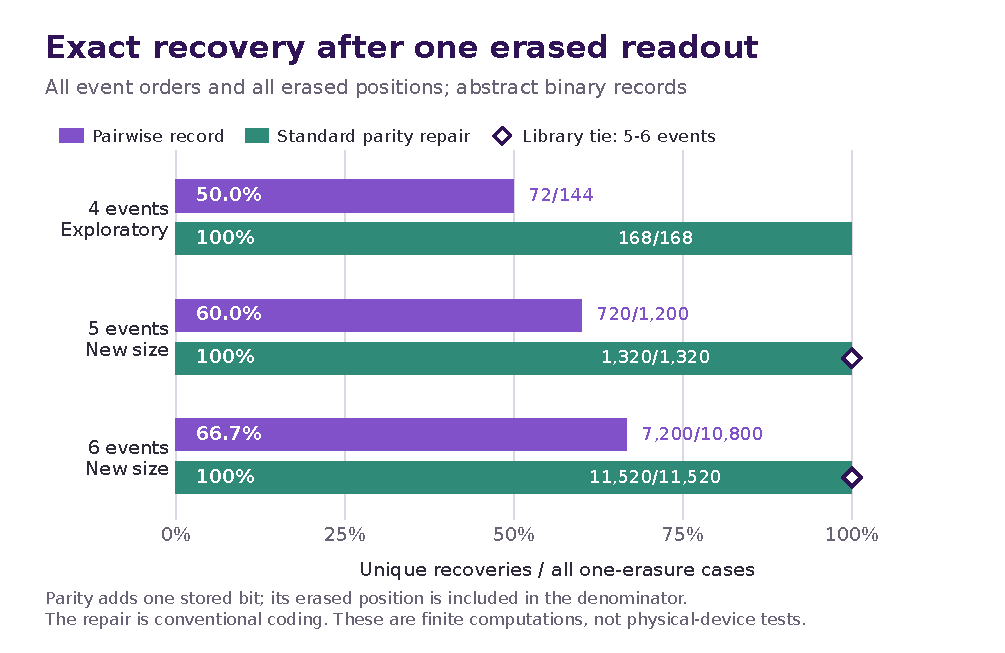
\includegraphics{../figures/figure-1-erasure-recovery.pdf}

\emph{Figure 1. Exhaustive abstract-code results. Bare pairwise records
recover 50\%, 60\% and 66.67\% of uniformly enumerated single-erasure
cases at n = 4, 5 and 6. Standard XOR parity recovers all declared
cases. The conventional identical-information library comparator ties on
the new-size checks; a separate bitset oracle independently verifies the
saved recovery sets. These are finite computations, not physical-device
reliability measurements.}

\hypertarget{repair-resource-bounds-and-negative-cases}{%
\subsection{5.2 Repair, resource bounds and negative
cases}\label{repair-resource-bounds-and-negative-cases}}

Append one bit equal to the XOR of the \(m\) pairwise bits. When one
known bit is erased, the surviving parity equation determines it; if
parity itself is erased, the original pairwise record remains intact. At
four events, the augmented abstract code recovers all 168
history/erasure cases. This is classical parity applied to a new
research connection. Its correctness does not make the coding principle
novel. {[}12, 31{]}

A duplication baseline requires \(2m\) stored bits within the restricted
class that stores only copies of individual pairwise comparisons. Every
pair can be adjacent in some history, so each must have at least two
copies to survive an arbitrary single erasure. The parity code uses
\(m+1\) logical bits. This comparison counts logical readouts; it is not
a lower bound for arbitrary encodings or a proof of lower physical cost.
A physical parity element could require couplers, ancillas, routing,
fabrication tolerances, energy or readout mechanisms absent from the
logical count.

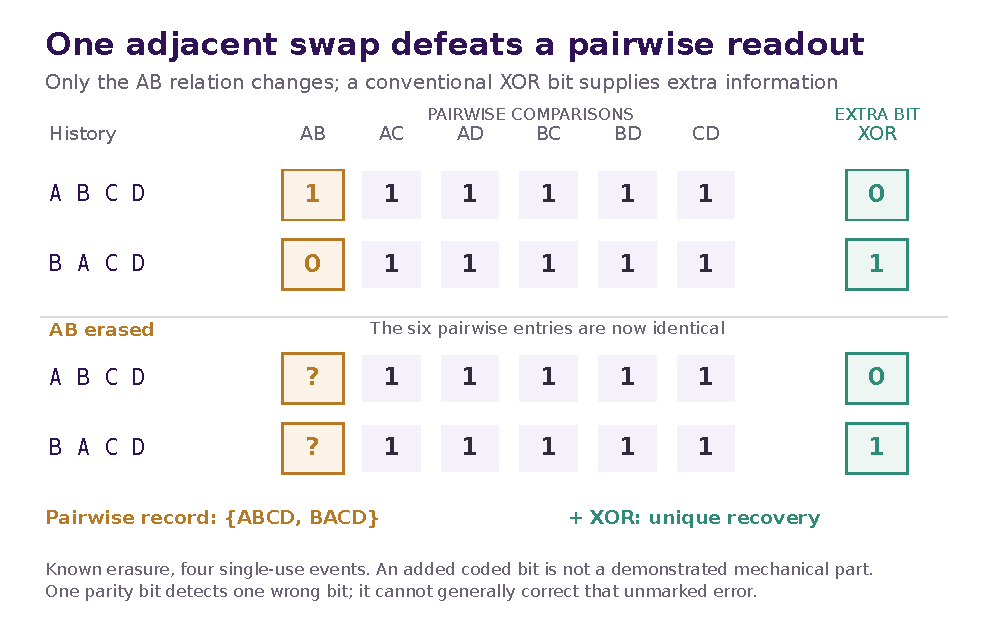
\includegraphics{../figures/figure-2-adjacent-swap.pdf}

\emph{Figure 2. ABCD and BACD differ only in the AB comparison. Removing
that comparison makes their bare readouts identical. An additional
conventional parity bit separates the two abstract codewords. The
diagram identifies the information requirement; it does not supply a
fabricated parity mechanism.}

The source and configuration were frozen before fresh-size enumeration.
At five events, bare recovery is 720/1,200 versus parity recovery of
1,320/1,320. At six events, the corresponding results are 7,200/10,800
and 11,520/11,520. The denominators differ because the augmented code
has one additional erasable position. A separate bitset-intersection
implementation checked all 198,840 enumerated recovery cases without
disagreement; another check verified 24,000 duplication cases. The
ordinary library containing the identical coding information ties on all
12,840 single-erasure cases at the new sizes. {[}31{]}

The preserved failures delimit the result. With two erasures, 1,560 of
6,600 five-event cases and 13,680 of 86,400 six-event cases remain
ambiguous under parity. All 12,840 tested single-bit substitutions are
detected, but a single parity check cannot generally correct an unknown
flipped bit. Erasing parity while flipping AB can silently change
ABCDE(F) into BACDE(F); flipping AB and AC can produce BCADE(F) with
parity still satisfied. These cases lie outside the promised
one-known-erasure model and are retained so that successors cannot
quietly generalize the guarantee.

The new-size checks establish implementation consistency on fresh finite
tasks. The general coding argument and the four-event design were
already known before their execution. Accordingly, this is technical
transfer of a known procedure, not learned independent competence,
prospective foresight or numerical retained Alpha.

\hypertarget{a-second-construction-deterministic-internal-races-order-sensitive-inputs}{%
\section{6. A second construction: deterministic internal races,
order-sensitive
inputs}\label{a-second-construction-deterministic-internal-races-order-sensitive-inputs}}

\hypertarget{exact-hysteron-model}{%
\subsection{6.1 Exact hysteron model}\label{exact-hysteron-model}}

The next search refinement sought a physically interpretable
distinction: internal switching order should not alter the result, while
the order of external events should. The constructed model contains
binary states \(s_i\), a held input vector \(h\), and effective fields

\[
H_i(s,h)=h_i+\sum_j C_{ij}s_j.
\]

An inactive bit may switch on when \(H_i\geq1.00\); an active bit may
switch off when \(H_i\leq-0.80\). Every allowed single-bit update choice
is explored. No update priority is used to manufacture determinism.
Nominal calculations use exact integer-scaled values. {[}32{]}

For the four-bit state \((x,y,z,w)\), only \(C_{xz}=C_{zx}=0.60\) and
\(C_{yw}=C_{wy}=0.60\) are nonzero. Pulse A is \((1.20,0,0,0.60)\), and
pulse B is \((0,1.20,0.60,0)\). Each is held until settling and followed
by zero input. C holds A+B simultaneously; R applies \((-2,-2,-2,-2)\)
until settling and then returns to zero. Two- and three-bit projections
are evaluated as separate models. An independent Boolean recurrence
supplies the semantic oracle:

\[
x'=x\lor a,\quad y'=y\lor b,\quad
z'=z\lor[b\land(x\lor a)],\quad
w'=w\lor[a\land(y\lor b)].
\]

R clears the state. Under the declared exactly-once two-event
interpretation, AB produces 1110 and BA produces 1101. C, ABA and BAB
all produce 1111. The collisions are central: the model cannot
reconstruct full history or uniquely identify simultaneous events.
Arbitrary finite-duration overlaps, thermal activation and physical
switching dynamics are outside its settled-input abstraction. {[}32{]}

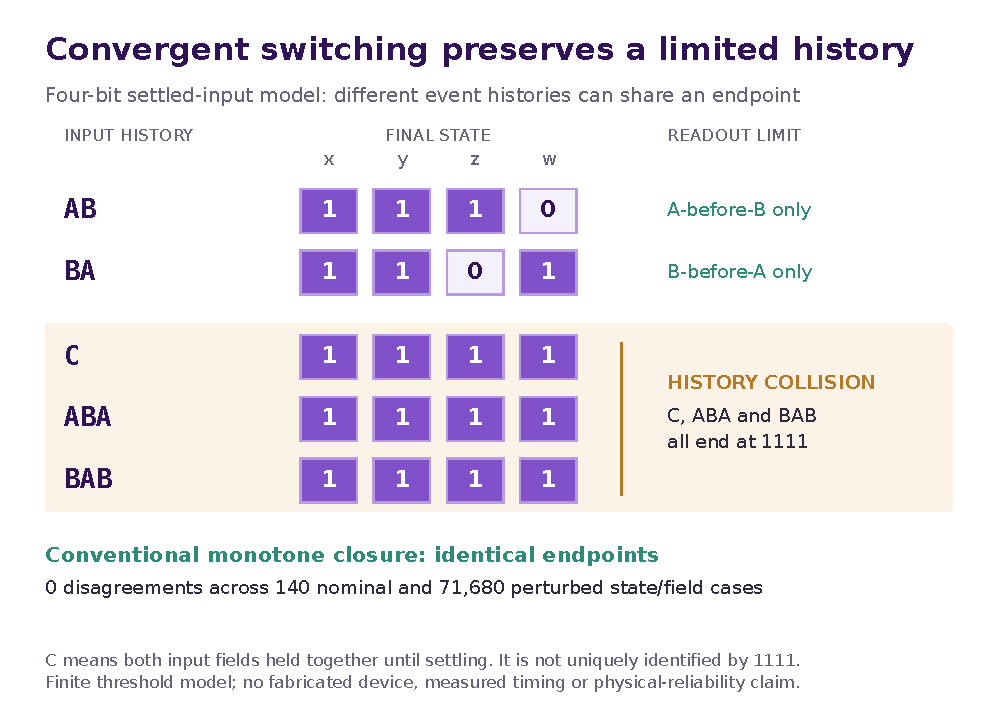
\includegraphics{../figures/figure-3-confluence-collisions.pdf}

\emph{Figure 3. Four-bit abstract hysteron readouts distinguish AB from
BA, while C, ABA and BAB collide at 1111. Every allowed internal update
schedule agrees within the declared model. A conventional
monotone-closure implementation gives identical results. This partial
event-order construction does not satisfy the original four-event
single-erasure offering.}

\hypertarget{why-it-works-and-why-it-does-not-earn-novelty}{%
\subsection{6.2 Why it works, and why it does not earn
novelty}\label{why-it-works-and-why-it-does-not-earn-novelty}}

Under A, B, C and zero, an active bit cannot switch off because fields
are nonnegative and the off threshold is negative. Every on-switch can
only increase neighboring fields. The process is therefore monotone on a
finite Boolean lattice and reaches the same least fixed point under
every maximal asynchronous update sequence. R forces all bits off. With
symmetric couplings, the coarse energy

\[
E(s;h)=-\sum_i h_i s_i-\sum_{i<j}C_{ij}s_i s_j
\]

strictly decreases at every allowed fixed-input switch. This supports
finite-model consistency; it supplies neither a continuous elastic
energy landscape nor a manufactured device. Different external vector
paths can still yield different final states. Internal confluence does
not imply that AB and BA commute, and this result does not overturn
scalar return-point-memory theory. {[}13, 32{]}

The confirmation includes all 140 nominal initial-state/held-field cases
across two, three and four bits; 5,461 words of length zero through six
per model over A/B/C/R; and 1,024 fresh seeded words of length one
through 64 per model. There are no oracle disagreements or nominal
nonconfluent cases. Parameter checks use 512 draws per dimension,
perturbing present symmetric edges, thresholds and nonzero drives by at
most 0.04, giving 71,680 state/field checks without disagreement.
Analytic interval margins also cover the continuous specified
perturbation box; the smallest required gated-activation margin is 0.08.
These are model checks, not independent physical trials or estimated
real failure rates. {[}32{]}

Unfavorable controls remain executable. Reducing each coupling from 0.60
to 0.35 destroys order discrimination. An antagonistic pair terminates
in either 01 or 10 depending on update order. An asymmetric feedback
pair cycles. The checker reports these behaviors. Eight acceptance tests
pass, including the negative controls.

The novelty verdict follows from stronger comparisons. Conventional
monotone closure matches the proposed dynamics exactly. Mechanical
counting, pattern recognition and reset already exist; systematic
transition-graph synthesis already exists; vectorial sequential memory
and autonomous event-order recorders are identified prior art. The
autonomous recorder comparison is especially useful because its
first-occurrence semantics are different from, and in some respects
stronger than, this recurrent-precedence state. Direct full text was
unavailable for the recent vectorial-memory preprint, so no detailed
performance comparison to it is asserted. A working threshold motif
earns a reference construction, not a new discovery claim. {[}9, 10,
13--15, 32{]}

\hypertarget{commercial-delivery-pricing-and-financing-for-the-same-offering}{%
\section{7. Commercial delivery, pricing and financing for the same
offering}\label{commercial-delivery-pricing-and-financing-for-the-same-offering}}

\hypertarget{scope-and-calibrated-assumptions}{%
\subsection{7.1 Scope and calibrated
assumptions}\label{scope-and-calibrated-assumptions}}

The commercial model concerns the original physically qualified
four-event chronology device with one known erased readout. It does not
sell the smaller latch, the abstract code or a generic diagnostic
service. There is no equivalent human-service market price to halve.
Instead, the comparison estimates a human-led development pathway and
models buyer value separately. All buyers, volumes, physical success
probabilities, device costs and prices are explicit scenarios; none is a
quote, sale or demonstrated willingness to pay. {[}33{]}

Two external anchors calibrate development labor. Job Bank reports
Montréal mechanical-engineer wages of CAD 30.43, 44.52 and 66.39 per
hour, with a 2024 reference period and a 19 November 2025 update. The
Bank of Canada's retrieved 26 October 2026 indicative rate is CAD 1.4025
per USD. Loading assumptions of 1.45, 1.70 and 2.10 produce USD 31.46,
53.96 and 99.41 per engineering hour. The loading factors, hours and
other costs are planning estimates, not source-reported project costs.
{[}26, 27, 33{]}

\Needspace{165pt}
\begingroup\small
\begin{longtable}[]{@{}
  >{\raggedright\arraybackslash}p{(\columnwidth - 6\tabcolsep) * \real{0.2000}}
  >{\raggedleft\arraybackslash}p{(\columnwidth - 6\tabcolsep) * \real{0.2667}}
  >{\raggedleft\arraybackslash}p{(\columnwidth - 6\tabcolsep) * \real{0.2667}}
  >{\raggedleft\arraybackslash}p{(\columnwidth - 6\tabcolsep) * \real{0.2667}}@{}}
\toprule\noalign{}
\begin{minipage}[b]{\linewidth}\raggedright
Development estimate
\end{minipage} & \begin{minipage}[b]{\linewidth}\raggedleft
Low
\end{minipage} & \begin{minipage}[b]{\linewidth}\raggedleft
Central
\end{minipage} & \begin{minipage}[b]{\linewidth}\raggedleft
High
\end{minipage} \\
\midrule\noalign{}
\endhead
\bottomrule\noalign{}
\endlastfoot
Engineering hours & 400 & 900 & 2,200 \\
Physical test hours & 200 & 500 & 1,500 \\
External prototypes, tooling and tests & \$18,000 & \$65,000 &
\$220,000 \\
Assumed duration & 3 months & 9 months & 18 months \\
Human-led total H & \$37,447 & \$141,170 & \$576,411 \\
Expert AI, no labor benefit E0 & \$38,054 & \$141,792 & \$577,056 \\
\end{longtable}
\endgroup

Physical test labor is costed at assumed USD 32, 45 and 65 per hour.
Research financing uses 10\% annually on an assumed average
half-deployed balance over the stated duration. Fifteen percent of
engineering cost represents failed screens already inside the total. The
central E0 total consists of \$48,567 engineering, \$22,500 physical
testing, \$65,000 external work, \$600 inference/tools and \$5,125
financing. The \$600 is a scenario allowance: 20 million input and four
million output tokens at the documented \texttt{gpt-6-astra} rates yield
\$400, plus \$200 tools and compute. It is not a provider invoice.
{[}28, 33{]}

E0 assumes \textbf{no} AI reduction in engineering hours or increase in
physical success. Hypothetical 25\% and 50\% engineering-hour reductions
are sensitivities, with physical testing unchanged. A high human R\&D
estimate therefore cannot silently become evidence that an AI pathway is
cheaper, faster or more likely to work.

\hypertarget{buyer-participation-and-the-best-tested-arrangement}{%
\subsection{7.2 Buyer participation and the best tested
arrangement}\label{buyer-participation-and-the-best-tested-arrangement}}

For each simulated buyer, device value combines assumed avoided losses
and staff savings, less false-alarm costs. The model assigns 70\%
prevented-loss benefit, but a passive record read after an event cannot
undo its damage. A downstream decision---such as disposition, future
prevention or adjudication---and its timing must be specified before
this becomes calibrated value. A manual outside option receives its own
assumed loss avoidance, staff saving and \$3 per-unit cost. Incremental
value is the positive difference between device value and the best
modeled outside option. Buyers participate only when effective price
plus the financing cost of any deposit is at most 70\% of that
incremental value. The remaining surplus supplies an explicit
participation margin; the rule is an assumption, not an elicited demand
curve or a truthful mechanism. {[}33{]}

The tested list-price grid is \$2, \$3, \$4, \$5, \$6, \$8, \$10, \$12,
\$16 and \$20. Payment policies are net 30 or a 20\% deposit with a 5\%
price discount. Deposit financing is charged to buyers at an assumed
10\% annual rate for thirty days. The supplier's credit-loss model
distinguishes postpaid exposure. A lower effective price can increase
participation while a deposit reduces financing pressure; raising prices
never holds demand artificially fixed.

Development uses 128 worlds. Policies were saved before a fresh
confirmation seed generated 512 worlds for each of three scenarios.
Capacity is capped at 120,000 devices annually. Potential buyers number
18, 40 or 70, with central per-buyer volumes of 2,000, 3,000 or 3,500
respectively; reachability, buyer value, demand, volume and unit cost
vary under the declared distributions. The selected policies are the
best tested policies for this model and grid, not globally optimal
real-world prices. {[}33{]}

\Needspace{160pt}
\begingroup\small
\begin{longtable}[]{@{}
  >{\raggedright\arraybackslash}p{(\columnwidth - 8\tabcolsep) * \real{0.1667}}
  >{\raggedright\arraybackslash}p{(\columnwidth - 8\tabcolsep) * \real{0.1667}}
  >{\raggedleft\arraybackslash}p{(\columnwidth - 8\tabcolsep) * \real{0.2222}}
  >{\raggedleft\arraybackslash}p{(\columnwidth - 8\tabcolsep) * \real{0.2222}}
  >{\raggedleft\arraybackslash}p{(\columnwidth - 8\tabcolsep) * \real{0.2222}}@{}}
\toprule\noalign{}
\begin{minipage}[b]{\linewidth}\raggedright
Confirmation scenario
\end{minipage} & \begin{minipage}[b]{\linewidth}\raggedright
Selected list price and terms
\end{minipage} & \begin{minipage}[b]{\linewidth}\raggedleft
Mean annual units if qualified
\end{minipage} & \begin{minipage}[b]{\linewidth}\raggedleft
Mean annual operating profit if qualified
\end{minipage} & \begin{minipage}[b]{\linewidth}\raggedleft
Expected project profit after central E0 development
\end{minipage} \\
\midrule\noalign{}
\endhead
\bottomrule\noalign{}
\endlastfoot
Conservative & \$4, net 30 & 2.9 & −\$73,910 & −\$160,270 \\
Central & \$5; 20\% deposit, 5\% discount & 58,113 & \$20,979 &
−\$131,303 \\
Favorable & \$8; 20\% deposit, 5\% discount & 96,034 & \$417,868 &
\$171,609 \\
\end{longtable}
\endgroup

The assumed physical-qualification probabilities \(q\) are 0.25, 0.50
and 0.75 respectively. Expected project profit is
\(q\,\mathbb{E}[\Pi_{\mathrm{operation}}]-A\), where A is the
development total and the operating branch is entered only after
qualification. The probabilities are not inferred from the code or
hysteron checks. Conservative participation almost entirely fails; 511
of 512 worlds have no sales. In the central scenario, 196 of 512
qualified-operation worlds lose money. These failures stay in the
evidence rather than disappearing behind an average. {[}33{]}

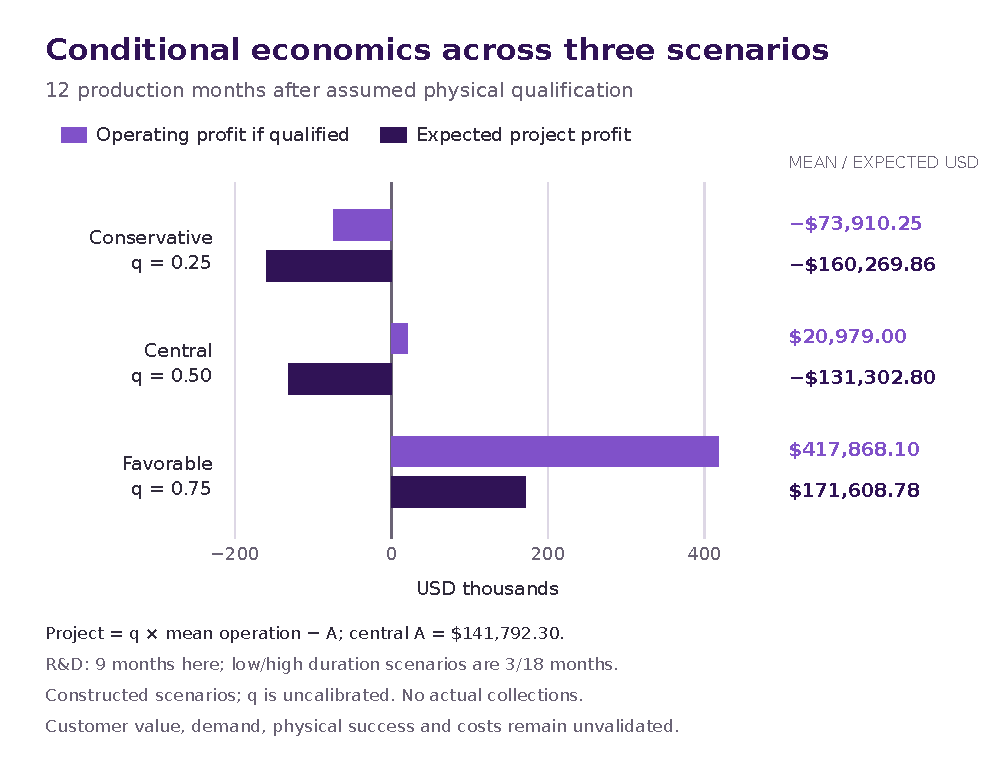
\includegraphics{../figures/figure-4-conditional-economics.pdf}

\emph{Figure 4. Frozen confirmation economics for the same hypothetical
four-event chronology offering. Operating profit assumes a qualified
product and twelve production months. Expected project profit is the
stipulated physical-success probability times mean operating profit,
minus central development cost; it is not an annualized return or a
sampled project-world mean. Probabilities, customer value and cost
adequacy remain unvalidated. No actual collections occurred.}

\hypertarget{favorable-case-accounts-and-unresolved-cost-scope}{%
\subsection{7.3 Favorable-case accounts and unresolved cost
scope}\label{favorable-case-accounts-and-unresolved-cost-scope}}

The favorable result is a pre-tax scenario calculation over development
plus one operating year, not an after-tax return or net present value.
Its 75\% success assumption and central \$141,792 development estimate
yield \(0.75\times417,868-141,792=171,609\) expected project profit.
Qualification failures and adverse commercial worlds still produce 137
losses among 512 simulated projects. The project-profit fifth and
ninety-fifth percentiles are −\$141,792 and \$437,756. These are
scenario quantiles, not empirical confidence intervals. {[}33{]}

\begingroup\small
\begin{longtable}[]{@{}
  >{\raggedright\arraybackslash}p{(\columnwidth - 4\tabcolsep) * \real{0.3000}}
  >{\raggedleft\arraybackslash}p{(\columnwidth - 4\tabcolsep) * \real{0.4000}}
  >{\raggedright\arraybackslash}p{(\columnwidth - 4\tabcolsep) * \real{0.3000}}@{}}
\toprule\noalign{}
\begin{minipage}[b]{\linewidth}\raggedright
Favorable qualified-operation account
\end{minipage} & \begin{minipage}[b]{\linewidth}\raggedleft
Mean USD
\end{minipage} & \begin{minipage}[b]{\linewidth}\raggedright
Interpretation
\end{minipage} \\
\midrule\noalign{}
\endhead
\bottomrule\noalign{}
\endlastfoot
Customer incremental value & \$1,326,650 & Value above the modeled
outside option, before price \\
Customer remaining surplus & \$595,594 & After price and prepayment
financing \\
Gross recognized revenue & \$729,856 & 96,034 units at effective price
\$7.60, subject to rounding \\
Collected cash & \$724,017 & After modeled credit losses and collection
runoff \\
Production and delivery & \$153,144 & Materials, fabrication, QA,
packaging/shipping, support/recovery \\
Customer acquisition & \$18,117 & Assumed acquisition expenditure \\
Warranty expense and credit loss & \$20,436 & \$14,597 warranty plus
\$5,839 credit loss \\
Contribution before overhead/finance & \$538,159 & Revenue less the
preceding variable/business charges \\
Fixed overhead and financing & \$120,290 & \$120,000 overhead plus \$290
operating finance \\
Annual operating profit & \$417,868 & Before the separately reported
originating development cost \\
Warranty liquidity reserve & \$21,896 & Reserved cash, not a second
warranty expense \\
Available after reserve and debt & \$395,972 & Conditional operating
cash; not actual growth funds \\
\end{longtable}
\endgroup

Unit production cost is decomposed into materials 40\%, fabrication
25\%, quality assurance 15\%, packaging/shipping 12\%, and
support/recovery 8\%. These are broad allowances, not an evidenced
complete bill of materials. Failed-prospect effort, yield/rework,
equipment, qualification, rights, insurance and exceptional returns are
unscoped. The 8\% support/recovery allocation may overlap the separate
warranty charge; internal physical-test labor and external testing also
lack task-level separation. Arithmetic consistency cannot establish that
real costs are complete or counted once. Fixed overhead and acquisition
are separate model entries. The twelve-month delivery model includes a
thirteenth month for receivable and warranty runoff. Deposits,
production and assumed acceptance occur sequentially within a monthly
bucket. The thirty-day lead is a buyer opportunity-cost assumption, not
dated seller cash evidence. Deposits become revenue only at assumed
acceptance; credit principal is financing, not revenue. Warranty expense
is 2\% of revenue, while a distinct 3\% liquidity reserve affects
available cash without being expensed twice. {[}33{]}

A revolving facility at an assumed 10\% annual rate covers operating
cash deficits. In the favorable case, mean peak credit is \$31,756.
Adding central development gives mean capital required of \$173,548,
with a ninety-fifth percentile of \$179,382. These are period-end
requirements under coarse monthly timing, not committed capital:
intramonth peaks, procurement leads, sales ramps, refunds and delayed
acceptance are unresolved. Actual collections, deliveries, recognized
revenue and token receipts are all zero. The actual full attributable
session cost is unknown, so no actual profit or available growth fund is
asserted. {[}33, 34{]}

\hypertarget{robustness-losses-and-the-development-decision}{%
\subsection{7.4 Robustness, losses and the development
decision}\label{robustness-losses-and-the-development-decision}}

At the favorable base assumptions, the break-even qualification
probability is approximately 0.339. This threshold holds the modeled
operating distribution and central development cost fixed. Central
operating economics would require \(q>1\) to repay that development cost
within the modeled horizon. Higher R\&D costs can overturn the favorable
case: the high E0 development estimate produces approximately −\$263,655
expected project profit; even an assumed 50\% engineering-hour reduction
leaves it negative. {[}33{]}

An exploratory demand/cost grid keeps the selected policies fixed.
Twenty-four of 42 favorable grid cells have both positive expected
project profit and a positive fifth-percentile annual operating profit;
no central or conservative cell does. At half base demand and unchanged
unit cost, favorable annual operating profit remains approximately
\$160,565, yet expected project profit becomes −\$21,368. At 75\% demand
and 1.5 times unit cost, expected project profit is about \$41,179.
These bounds clarify which economic assumptions deserve early
calibration. They are not a demonstrated robust market region. {[}33{]}

A same-team independent Decimal audit checked 16,968 identities or
comparisons across all 1,536 confirmation worlds; the saved
reconstructed auditor adds 12,543 numeric checks. Residuals remain below
\$0.000001. The original inline command was not preserved; its
reconstructed source and changed rounding residual are explicitly
documented. This validates arithmetic, failure preservation and
physical-work invariance, not actionable benefit, real cost completeness
or disjoint cost scope. The model-review record preserves these material
limitations without changing the frozen results. {[}33{]} All actual
decisions remain \textbf{HOLD: unqualified physical offering and failed
novelty gate}. Avoiding future expenditure does not erase sunk research
cost.

\hypertarget{post-result-cost-headroom}{%
\subsection{7.5 Post-result cost
headroom}\label{post-result-cost-headroom}}

An additional exploratory accounting stress, performed after the frozen
results, asks how much unscoped cost the favorable case could absorb
without changing buyer behavior, prices, qualification or financing. Let
\(\Delta A\) be additional originating cost and \(\Delta O\) additional
annual qualified-operation expense. Positive expected project profit
requires \(\Delta A+0.75\Delta O<171{,}608.78\) USD. Keeping its
fifth-percentile annual operating result positive additionally requires
\(\Delta O<191{,}951.16\) USD for a constant annual expense. The central
case has no nonnegative added-cost region. These are accounting
boundaries inside the constructed scenario, not estimates of omitted
costs, evidence of cost completeness or a behavioral reoptimization.
Induced financing, delays and demand responses require a new model. The
exact derivation and provenance are in
\nolinkurl{results/cost-headroom-exploratory.json} and
\nolinkurl{src/cost_headroom.py}. Actual HOLD is unchanged. {[}33{]}

\hypertarget{frontier-models-operational-alpha-and-the-foresight-comparison}{%
\section{8. Frontier models, Operational Alpha and the foresight
comparison}\label{frontier-models-operational-alpha-and-the-foresight-comparison}}

Official documentation was checked on 27 October 2026. The inventory
records exact identifiers, rates, proposed configurations and access
limitations. It establishes suitable experiment candidates, not that the
present account had every listed API entitlement or that provider
benchmarks predict success on this offering. No paid provider API
mission experiment was run. {[}28--30{]}

\Needspace{180pt}
\begingroup\small
\begin{longtable}[]{@{}
  >{\raggedright\arraybackslash}p{(\columnwidth - 6\tabcolsep) * \real{0.2308}}
  >{\raggedright\arraybackslash}p{(\columnwidth - 6\tabcolsep) * \real{0.2308}}
  >{\raggedright\arraybackslash}p{(\columnwidth - 6\tabcolsep) * \real{0.2308}}
  >{\raggedleft\arraybackslash}p{(\columnwidth - 6\tabcolsep) * \real{0.3077}}@{}}
\toprule\noalign{}
\begin{minipage}[b]{\linewidth}\raggedright
Exact model identifier
\end{minipage} & \begin{minipage}[b]{\linewidth}\raggedright
Proposed role
\end{minipage} & \begin{minipage}[b]{\linewidth}\raggedright
Proposed reasoning/output configuration
\end{minipage} & \begin{minipage}[b]{\linewidth}\raggedleft
USD per million input/output tokens
\end{minipage} \\
\midrule\noalign{}
\endhead
\bottomrule\noalign{}
\endlastfoot
\texttt{gpt-6-astra} & Discovery and difficult judgment & \texttt{max},
64,000 output cap & 10 / 50 \\
\texttt{gpt-6.1-sol} & Execution comparator & \texttt{high}, 32,000
output cap & 2 / 10 \\
\texttt{gpt-6.1-terra} & Computer-use execution candidate &
\texttt{high}, 32,000 output cap & 1 / 5 \\
\texttt{claude-fable-5-1} & Independent-family validation candidate &
Adaptive thinking, \texttt{max}, 64,000 cap & 10 / 50 \\
\texttt{claude-opus-5-5} & Implementation comparator & Adaptive
thinking, \texttt{high}, 64,000 cap & 4 / 20 \\
\texttt{gemini-4-argon} & Scientific reasoning candidate &
\texttt{high}, 65,536 output cap & 2 / 10 through 30 November 2026 \\
\end{longtable}
\endgroup

The inventory records context limits, selected provider tool
availability and the Google rate change scheduled for December. The
listed configurations are proposals, not executed mission
configurations; exact tool schema versions must be frozen before a
comparative provider run. OpenAI reasoning/tool proposals use the
Responses API and omit unsupported sampling controls. Actual cost logs
must include reasoning output, retries, verification and tool usage.
Closed weights, unrestricted consumer-subscription automation and
untested account access are not assumed.

Operational Alpha means E performing better than U with the
\textbf{same} frontier model, initial evidence, tools, reasoning limits
and total budget. Retained Alpha compares E+ with E after charging the
incremental retained capability. The present study implements expert
research practices---source construction, decomposition, exact
verification, adversarial controls and recovery---but contains no
controlled numerical E-versus-U result. H is a transparent development
estimate, not a recruited human team. Independent implementations were
produced within the same assistant-controlled team; they are not
independent model families or blinded human adjudicators. {[}31--35{]}

A prospective comparison should therefore be frozen before its next
discovery run. The proposed design uses identical need/resource packets
containing no intended opportunity, source access cutoffs, equal model
identifiers and monetary/token limits, and a fixed candidate budget.
Representative U receives a competent open-ended opportunity-search
instruction and the same available tools; E receives the expert
orchestration procedure. Expertise may change decomposition and
verification, but cannot obtain extra information or budget. Multiple
sessions and seed assignments should be specified in the frozen
protocol, rather than selected after favorable outputs appear.

Novelty, usefulness, technical feasibility and commercial plausibility
should be reviewed separately against predeclared criteria. Reviewers
should receive source-backed constructions without condition labels
where practical. Human experts should search the same packet if
recruited; otherwise the edition must report that the human comparison
is absent or explicitly modeled. The final test must include an
executable construction or decisive experiment, with fresh acceptance
cases hidden from the search sessions. Merely failing to mention an
opportunity in a baseline sample does not establish beyond-human
foresight. Historical replay would additionally require defensible
information cutoffs and leakage controls; none is claimed here.

\hypertarget{insight-nova-seed-fusionplan-and-mark-as-an-actual-connected-mechanism}{%
\section{9. Insight, Nova-Seed, FusionPlan and MARK as an actual
connected
mechanism}\label{insight-nova-seed-fusionplan-and-mark-as-an-actual-connected-mechanism}}

The integration copies and hashes forty unchanged adapter source/license
files and two additional unchanged scenario modules from the audited
repository snapshot. It executes native scenario analysis, Nova-Seed
cryptographic roundtripping, FusionPlan compilation and verification,
cost-ledger safeguards, and authority checks. This is a real local
integration with public fixtures, distinct from a narrative business
plan. {[}34, 35{]}

The native Insight scenario receives seven reviewer-supplied rejected
candidates and retrieves eight exact excerpts from their supplied
evidence. Each candidate has unit synthetic cost and zero eligibility
value. Across 128 possible subsets it selects none, produces no
schedule, and \texttt{makeGenome} refuses to create a venture genome.
Identical numeric coordinates place all seven candidates on the computed
nondominated frontier, which does not make them qualified. The numeric
setup records the completed review; it is not an independent semantic
novelty evaluation or proof that Insight discovered the rejection
unaided. The generic refusal suggestion to increase budget does not
override the actual reason: eligibility is zero despite every candidate
fitting the synthetic budget.

A separate research Nova-Seed preserves the negative result,
opportunity, original purpose, sources, uncertainty, rights scope,
transformation witness, evidence and next experiment. Native WebCrypto
encryption and authenticated decryption roundtrip the object; wrong
passphrases and modified commitments are rejected. A public fixture
passphrase establishes an inspectable test, not secrecy. Cryptographic
integrity shows that the object is unchanged, not that its scientific
claim is true.

The FusionPlan contains four executable milestone descriptions:
discovery, construction, economics and retention. Native Merkle
compilation and verification check committed fields. The fixture
allocates 100 base units of AGIALPHA per job, 400 total; these are local
test units, not USD, funded bounties or revenue. Dependencies, full
budgets, permissions, acceptance conditions and falsifiers are retained
in the research object. The native commitment format does not itself
enforce every wider research obligation.

Thirteen adapter checks pass. They include rejecting a substituted
acceptance metric, double-charged activities, treating unknown cost as
zero, unsupported capsule scope, unreviewed rights and production
admission based only on a valid local signature. A simulated identity
without live ENS authorization remains denied, and denial does not
consume the challenge. The public research artifact cannot be renamed to
fit an existing production capability's narrower approved scope. The
adapter emits an inspectable MARK review packet; MARK execution remains
\texttt{NOT\_EXECUTED}, and no minting, listing, trading, funds
movement, on-chain action or expanded permission occurs. {[}34{]}

These outcomes preserve the existing validator roles. The research
pipeline can archive a useful failed hypothesis while venture promotion
and production access remain closed. Native execution used Python
3.12.14 and Node 24.22.1; the production Node pin differs, so the local
checks are not a production release qualification.

\hypertarget{what-the-successor-inheritsand-what-it-must-earn}{%
\section{10. What the successor inherits---and what it must
earn}\label{what-the-successor-inheritsand-what-it-must-earn}}

The successor can inherit exact models, source-scoped claims,
counterexamples, configurations, a schedule-complete checker, an
independent decoding oracle and the complete commercial assumptions.
Each object has a version, provenance, dependencies, scope and failure
modes. The intended rights scope is public research code and
public-source metadata; external publications retain their own rights.
Secrets, customer material and protected evaluation answers are not part
of the capsule. {[}31--35{]}

Accounting separates A, originating delivery or research; B, additional
evaluation, extraction, retention, invocation and maintenance; and C,
optional extra research or Gym training. Necessary learning already
charged to A is not charged again in B. The present construction was
unpaid research, not learning acquired during an accepted paid job. The
actual native ledger marks originating and additional-validation
expenditure unknown, sets optional Gym execution to zero, and refuses to
calculate actual profit from incomplete costs.

The optional retained-service scenario adds \$2,500
extraction/validation and \$1,200 annual maintenance, or \$3,700. Ten
future missions would require an average \$370 incremental benefit per
mission to break even. The identical-information ordinary library
produces no observed acceptance improvement over the retained code.
Under the tested zero-incremental-saving case, the optional premium
retention investment loses \$3,700 and is rejected. Public preservation
remains useful; it is not evidence that maintaining a specialist
business is free or profitable. {[}33{]}

No model weights were trained, no Gym learning curve was measured and no
specialist superhuman claim is made. The fresh five- and six-event tasks
demonstrate the same known algorithm operating at new sizes. Remote
service access would likewise not establish that a recipient
independently acquired competence. The operational inheritance rule is:
\textbf{REUSE stable structure; RECHECK the new mission's meaning;
REGRANT authority separately.} Authenticated agent-network distribution
must use the actual authorization workflow; local fixture identities do
not grant access across \texttt{*.agent.agi.eth}.

The next challenge is a useful physical history property that existing
mechanical, finite-state and coding controls cannot satisfy under the
same complete resource budget. The inherited models help falsify
proposals; they do not establish that such a gap exists.

\hypertarget{the-smallest-useful-next-validation}{%
\section{11. The smallest useful next
validation}\label{the-smallest-useful-next-validation}}

The first next step is a bounded novelty-and-realizability challenge,
before a full hardware program. Specify one valuable history predicate,
its event and fault model, complete physical component budget,
permissible energy and readout mechanism. Ask a materials specialist to
compare it with the identified general hysteron-synthesis,
event-recorder and classical-code controls. A proposed advantage fails
if a conventional construction meets the same obligations at comparable
total resources.

If a functional gap survives, map the smallest motif to a calibrated
continuous potential or existing tunable-hysteron geometry. Check
metastable branches, actual ramps, damping, noise and reset; then
fabricate only the component needed to falsify the proposed physical
mechanism. This step would test physical feasibility. Fabricating the
already known parity or latch principle alone would not repair the
novelty deficit. The complete four-event erasure requirement remains the
product acceptance gate.

In parallel, a small scoped buyer interview can test whether the claimed
history changes a real decision, what outside option is used, and
whether the favorable model's incremental value and volume assumptions
are plausible. A quote can calibrate fabrication and test costs. These
activities refine a conditional model; they do not retroactively turn
simulated revenue into collections. Their budgets and permissions must
be separately authorized when needed.

The exact constructions, conventional ties and rejected opportunities
equip a successor to continue the search with its acceptance standard
intact.

\hypertarget{appendix-a.-reproducibility-and-evidence-map}{%
\section{Appendix A. Reproducibility and evidence
map}\label{appendix-a.-reproducibility-and-evidence-map}}

All paths below are relative to this study directory. The repository
edition contains source, frozen configurations, seeds, results, audit
records and figures. The core order-memory and confluence experiments
use Python's standard library; figure reproduction additionally uses
matplotlib. The integration requirements and exact upstream source lock
are separate from the scientific kernels.

\Needspace{180pt}
\begingroup\small
\begin{longtable}[]{@{}
  >{\raggedright\arraybackslash}p{(\columnwidth - 4\tabcolsep) * \real{0.3333}}
  >{\raggedright\arraybackslash}p{(\columnwidth - 4\tabcolsep) * \real{0.3333}}
  >{\raggedright\arraybackslash}p{(\columnwidth - 4\tabcolsep) * \real{0.3333}}@{}}
\toprule\noalign{}
\begin{minipage}[b]{\linewidth}\raggedright
Evidence
\end{minipage} & \begin{minipage}[b]{\linewidth}\raggedright
Reproduction entry point
\end{minipage} & \begin{minipage}[b]{\linewidth}\raggedright
Preserved output
\end{minipage} \\
\midrule\noalign{}
\endhead
\bottomrule\noalign{}
\endlastfoot
Four-event probe &
\nolinkurl{discovery/order-memory/mechanical_memory_probe.py} &
\texttt{mechanical\_memory\_probe.json} \\
Frozen new-size decoding &
\nolinkurl{discovery/order-memory/order_transfer_study.py} &
\nolinkurl{transfer_validation/transfer_results.json}, compressed case
stream \\
Hysteron confirmation & \nolinkurl{experiments/confluence/study.py};
\texttt{test\_study.py} & \texttt{results.json}, \texttt{freeze.json},
confirmation words \\
Economics & \nolinkurl{src/economics.py} with
\nolinkurl{config/economics.json} & Development, policy freeze,
confirmation worlds and sensitivity \\
Native integration & \nolinkurl{integration/run_adapter.py};
\texttt{run\_scenario.mjs} & Chronology and scenario run reports \\
\end{longtable}
\endgroup

Consult each component's README or reproduction notes for its working
directory and arguments. Frozen configurations must be preserved when
reproducing results; changing a model requires a new labeled experiment,
not overwriting the acceptance history. The order study freezes
source/configuration before n = 5/6 execution. Confluence freezes its
configuration before programmatic confirmation, after the design was
hand-derived. Economics freezes selected policies before fresh-seed
confirmation. These are distinct chronological guarantees and none makes
the overall adaptive search blind.

The economics development seed is \texttt{2026102701}; confirmation uses
\texttt{2026102702}. All 1,536 confirmation worlds are retained. An
interrupted disk-write artifact and its unchanged rerun are preserved.
Independent audit files document decoding and Decimal accounting checks.
Figures are generated by \nolinkurl{src/build_figures.py};
\nolinkurl{figures/caption_manifest.json} records their source data and
scope. Deterministic exhaustive counts need no sampling confidence
interval; commercial and perturbation scenarios do not become empirical
reliability estimates merely because many cases were run.

\hypertarget{appendix-b.-contributions-data-availability-and-publication-status}{%
\section{Appendix B. Contributions, data availability and publication
status}\label{appendix-b.-contributions-data-availability-and-publication-status}}

The author line follows the commissioned manuscript. The user supplied
the mission, novelty gate, research obligations and ecosystem
references. Assistant-controlled research agents supplied candidate
generation, source screening, mathematical formulations, code, controls,
economic scenarios, integration adapters and drafting. Separate agents
performed implementation audits, but shared the same controller and
evidence environment. No independent human expert study, external peer
review, live buyer trial or provider-controlled model comparison is
implied.

Data and code are supplied with this study, including failed cases and
the no-flagship decision. Scientific acceptance applies only to the
declared finite computations. Commercial figures are conditional
simulations. Production authorization remains denied. This manuscript is
a source draft for review; the canonical browser/PDF publication route
is coordinated with the existing owner. No merge, live canonical Pages
update or external publication is asserted by this document.

\small
\hypertarget{references-and-source-scope}{%
\section{References and source
scope}\label{references-and-source-scope}}

All online sources below were inspected or their specified metadata
checked during the 27 October 2026 study. Local evidence references
identify reproducible artifacts. Descriptions are scoped to the claims
used here.

\begin{enumerate}
\def\labelenumi{\arabic{enumi}.}
\tightlist
\item
  \textbf{Commissioned brief.} Exact supplied instructions,
  \nolinkurl{discovery/INITIAL_BRIEF.txt}. Primary task record,
  2026-10-27.
\item
  \textbf{MONTREAL.AI.}
  \href{https://github.com/MontrealAI/AGI-Alpha-Agent-v0}{AGI-Alpha-Agent-v0}
  and
  \href{https://github.com/MontrealAI/AGI-Alpha-Agent-v0/issues/4850}{coordination
  issue 4850}. Primary implementation and coordination records;
  inspected snapshot recorded in provenance.
\item
  \textbf{Transformational Intelligence.}
  \href{https://montrealai.github.io/AGI-Alpha-Agent-v0/Transformational_Intelligence.pdf}{Foundational
  paper}. Primary project research, inspected 2026-10-27.
\item
  \textbf{Invent the Economy.}
  \href{https://montrealai.github.io/AGI-Alpha-Agent-v0/Invent_the_Economy.pdf}{Foundational
  paper}. Primary project research, inspected 2026-10-27.
\item
  \textbf{Autonomous Enterprises: Build the Means of Building.}
  \href{https://montrealai.github.io/AGI-Alpha-Agent-v0/Autonomous_Enterprises.pdf}{Foundational
  paper}. Primary project research, inspected 2026-10-27.
\item
  \textbf{MONTREAL.AI commercial and retained-capability studies.}
  Repository primary papers:
  \href{https://github.com/MontrealAI/AGI-Alpha-Agent-v0/blob/main/docs/papers/agi-alpha-operational-economics-v1.pdf}{Complete
  Economics},
  \href{https://github.com/MontrealAI/AGI-Alpha-Agent-v0/blob/main/docs/papers/profitable-work-first.pdf}{Profitable
  Work First},
  \href{https://github.com/MontrealAI/AGI-Alpha-Agent-v0/blob/main/docs/papers/when-paid-work-teaches-the-network.pdf}{When
  Paid Work Teaches the Network}, and
  \href{https://github.com/MontrealAI/AGI-Alpha-Agent-v0/blob/main/docs/papers/network-learns-to-invent-v1.pdf}{The
  Network Learns to Invent}. Snapshot scope and corrections in the
  audit; no results imported.
\item
  \textbf{Operational Alpha v2.}
  \href{https://github.com/MontrealAI/AGI-Alpha-Agent-v0/blob/e5e4441aa7eb3b524edb1ba3152554baf44c8247/studies/agi-alpha-operational-alpha-v2/paper/Browser_Edition.md}{Browser
  edition at inspected commit}. Primary project study, 2026; local
  inspected record in provenance.
\item
  \textbf{Emergent disorder and mechanical memory in periodic
  metamaterials.}
  \href{https://www.nature.com/articles/s41467-024-47780-w}{Nature
  Communications}, 2024. Primary journal article;
  \href{https://pmc.ncbi.nlm.nih.gov/articles/PMC11109184/}{open full
  text}.
\item
  \textbf{Liu et al.~Controlled pathways and sequential information
  processing in serially coupled mechanical hysterons.}
  \href{https://doi.org/10.1073/pnas.2308414121}{PNAS}, 2024. Primary
  journal article;
  \href{https://pmc.ncbi.nlm.nih.gov/articles/PMC11145188/}{open full
  text}.
\item
  \textbf{Teunisse and van Hecke. Transition graphs of interacting
  hysterons: structure, design, organization and statistics.}
  \href{https://doi.org/10.1098/rsos.250753}{Royal Society Open
  Science}, 2025-09-24. Primary full text:
  \href{https://pmc.ncbi.nlm.nih.gov/articles/PMC12457013/}{PMC}.
\item
  \textbf{Paulsen. Mechanical hysterons with tunable interactions of
  general sign.}
  \href{https://www.nature.com/articles/s41467-026-70913-2}{Nature
  Communications}, 2026-04-11. Primary journal article.
\item
  \textbf{Hamming. Error Detecting and Error Correcting Codes.}
  \href{https://www.nokia.com/bell-labs/publications-and-media/publications/error-detecting-and-error-correcting-codes/}{Bell
  System Technical Journal record}, 1950. Primary foundational paper;
  \href{https://zoo.cs.yale.edu/classes/cs323/doc/Hamming.pdf}{PDF
  copy}.
\item
  \textbf{Sethna et al.~Hysteresis and hierarchies: Dynamics of
  disorder-driven first-order phase transformations.}
  \href{https://doi.org/10.1103/PhysRevLett.70.3347}{Physical Review
  Letters}, 1993;
  \href{https://arxiv.org/html/cond-mat/9210018v1}{primary preprint}.
\item
  \textbf{Meulblok and van Hecke.}
  \href{https://arxiv.org/abs/2607.11179}{Vectorial-input mechanical
  memory preprint}, July 2026. Primary abstract inspected; direct full
  text unavailable during the probe.
\item
  \textbf{Cardelli.}
  \href{https://link.springer.com/chapter/10.1007/978-981-19-9891-1_17}{Autonomous
  event-order recording}, 2023. Primary research chapter, full text
  inspected; first-occurrence semantics differ from this study's
  recurrent-precedence latch.
\item
  \textbf{Shetty and Braga-Neto. LLM-IDEA: Identifiability-Driven
  Experimental Agent for Autonomous Discovery of Mechanistic World
  Models.} \href{https://arxiv.org/abs/2610.11253}{Primary preprint},
  2026-10-08.
\item
  \textbf{Rassouli, Rosas and Gunduz. Data Disclosure under Perfect
  Sample Privacy.} \href{https://arxiv.org/abs/1904.01711}{Primary
  preprint}, 2019-04-02. Its distributional privacy notion is not
  unrestricted side-information robustness.
\item
  \textbf{Zhao et al.~From Mathematical to Executable Certificates for
  Machine Unlearning.} \href{https://arxiv.org/abs/2610.02268}{Primary
  preprint record}, 2026-10-01. Metadata inspected; detailed technical
  performance not used.
\item
  \textbf{Hou et al.~Experimental realization of a full-band wave
  antireflection based on temporal taper metamaterials.}
  \href{https://www.nature.com/articles/s42005-026-02500-2}{Communications
  Physics}, 2026-01-15. Primary full text.
\item
  \textbf{Catalytic resonance theory: parallel reaction pathway
  control.}
  \href{https://pubs.rsc.org/en/content/articlehtml/2020/sc/c9sc06140a}{Chemical
  Science}, 2020. Primary article;
  \href{https://pmc.ncbi.nlm.nih.gov/articles/PMC8152411/}{open full
  text}.
\item
  \textbf{Rajput and Pahlavan. Fluidic Hysterons and Memory in Flow
  Networks.}
  \href{https://journals.aps.org/prx/abstract/10.1103/hh4n-pw7w}{Physical
  Review X}, 2026-10-09. Primary abstract inspected.
\item
  \textbf{Ahrar, Raje, Lee and Hui. Pneumatic computers for embedded
  control of microfluidics.}
  \href{https://pmc.ncbi.nlm.nih.gov/articles/PMC10413662/}{Science
  Advances full text}, 2023. DOI: 10.1126/sciadv.adg0201.
\item
  \textbf{Generalizing multiple memories from a single drive: The
  hysteron latch.}
  \href{https://pmc.ncbi.nlm.nih.gov/articles/PMC11778092/}{Primary full
  text}, 2025.
\item
  \textbf{Ali et al.~Materializing split, mixed, and three-body
  interactions using rotor-based mechanical hysterons.}
  \href{https://arxiv.org/abs/2607.21974}{Primary preprint}, 2026-07-24.
  Abstract inspected.
\item
  \textbf{Thakkar, Rivas-Padilla and Arrieta. Visco-Bits:
  temporal-coding-inspired viscoelastic metamaterial for mechanical
  memory expansion.} \href{https://doi.org/10.1039/d6mh00721j}{Primary
  journal record}, 2026;
  \href{https://pubmed.ncbi.nlm.nih.gov/42525443/}{metadata}. Year used
  because online and issue dates differ.
\item
  \textbf{Government of Canada, Job Bank. Mechanical engineer wages,
  Montréal.}
  \href{https://www.jobbank.gc.ca/marketreport/wages-occupation/2757/22447}{Official
  wage report}. Reference period 2024; updated 2025-11-19; retrieved
  2026-10-27.
\item
  \textbf{Bank of Canada. Daily exchange rates.}
  \href{https://www.bankofcanada.ca/rates/exchange/daily-exchange-rates/}{Official
  indicative rates}. USD observation for 2026-10-26, retrieved
  2026-10-27; not a transaction quote.
\item
  \textbf{OpenAI.} Official
  \href{https://developers.openai.com/api/docs/models}{models},
  \href{https://developers.openai.com/api/docs/guides/latest-model}{latest-model
  guide} and
  \href{https://developers.openai.com/api/docs/pricing}{pricing}.
  Retrieved 2026-10-27; exact inventory in
  \nolinkurl{provenance/models_2026-10-27.json}.
\item
  \textbf{Anthropic.} Official
  \href{https://platform.claude.com/docs/en/models/fable-5-1/overview}{Fable
  5.1},
  \href{https://platform.claude.com/docs/en/models/opus-5-5/overview}{Opus
  5.5} and
  \href{https://platform.claude.com/docs/en/build-with-claude/effort}{effort
  configuration}. Retrieved 2026-10-27; access not tested.
\item
  \textbf{Google.} Official
  \href{https://ai.google.dev/gemini-api/docs/models/gemini-4-argon}{Gemini
  4 Argon},
  \href{https://ai.google.dev/gemini-api/docs/latest-model}{latest-model
  documentation} and
  \href{https://ai.google.dev/gemini-api/docs/pricing}{pricing}.
  Retrieved 2026-10-27; time-limited price recorded.
\item
  \textbf{This study: discovery and order-memory evidence.}
  \nolinkurl{discovery/order-memory/discovery_record.json},
  \texttt{mechanical\_memory\_probe.json},
  \nolinkurl{transfer_validation/transfer_results.json}, compressed
  cases, theory notes and independent adversarial review. Primary
  executable research, 2026-10-27.
\item
  \textbf{This study: confluence evidence.}
  \nolinkurl{experiments/confluence/README.md}, model and configuration,
  freeze, source, tests and \texttt{results.json}. Primary executable
  research, 2026-10-27.
\item
  \textbf{This study: commercial evidence.}
  \nolinkurl{config/economics.json}, \nolinkurl{src/economics.py},
  \nolinkurl{results/economics-results.json}, frozen policy, all worlds,
  sensitivity, independent Decimal audits and
  \nolinkurl{results/economics-model-review-v1.json}. Primary conditional
  simulation, 2026-10-27.
\item
  \textbf{This study: native workflow evidence.}
  \nolinkurl{integration/README.md}, \texttt{SCENARIO\_README.md}, source
  lock and reports under \nolinkurl{integration/results/}. Primary local
  execution with fixture identities, 2026-10-27.
\item
  \textbf{This study: ecosystem audit.} \nolinkurl{provenance/AUDIT.md},
  \texttt{source\_manifest.json} and inspected Operational Alpha record.
  Primary provenance and scope audit, 2026-10-27.
\end{enumerate}

\end{document}
